\documentclass[main.tex]{subfiles}

\begin{document}

\chapter{Localização de ponto}

Neste capítulo analisaremos uma variação do problema de localização de ponto (point location)~\cite{SarnakT1986}, e mostraremos uma solução utilizando a ABB persistente descrita no Capítulo~\ref{cap:rubronegra_persist}.

Dado um conjunto de polígonos~${\{P_1, \ldots, P_k\}}$ tal que nenhum dos polígonos se intersecta, queremos responder múltiplas consultas do seguinte tipo: Dado um ponto~$p$, determine~$i$ tal que~${p \in P_i}$ ou diga que tal~$i$ não existe.

A Figura~\ref{fig:exemplo_pl} mostra um exemplo do problema com três polígonos. Os pontos de consulta estão coloridos com a cor do polígono a qual pertencem, ou pretos se não pertencem a nenhum dos polígonos.


\begin{figure}
\centering
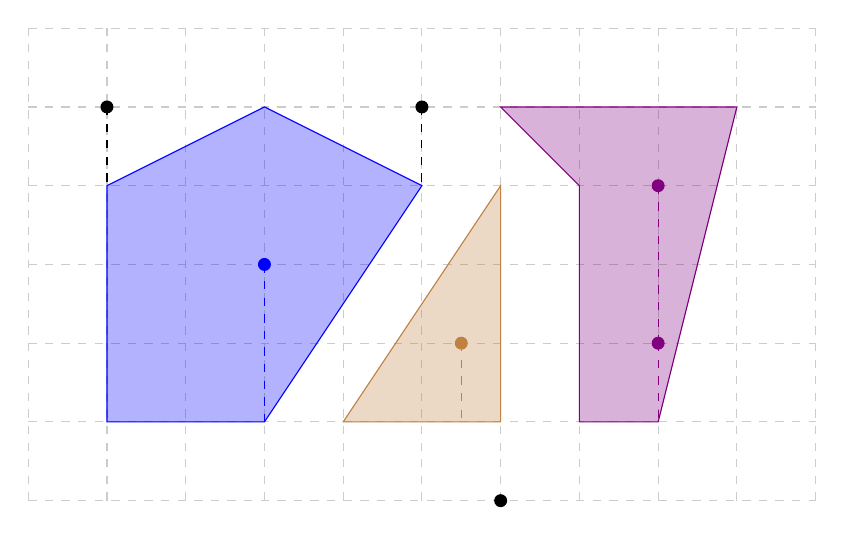
\begin{tikzpicture}[]

\newcounter{size}
\newcommand\polyg[2]{
	\setcounter{size}{0}
	\foreach \point [count=\i] in #1 {
		\stepcounter{size}
		\node[coordinate] (p1-\i) at \point {};
	}
	\fill[#2, opacity=0.3] (p1-1) \foreach \i in {2, ..., \value{size}} {-- (p1-\i)} -- cycle;
	\draw[#2, opacity=1] (p1-1) \foreach \i in {2, ..., \value{size}} {-- (p1-\i)} -- cycle;
}

\draw[opacity=0.2, dashed] (-8, 0) grid (2, 6);

\polyg {{(-7, 4), (-5, 5), (-3, 4), (-5, 1), (-7, 1)}}{blue};
\polyg {{(-2, 5), (-1, 4), (-1, 1), (0, 1), (1, 5)}}{violet};
\polyg {{(-2, 4), (-4, 1), (-2, 1)}}{brown};

\newcommand\drawpts[2]{ \foreach \point in #1 { \draw[fill=#2, color=#2] \point circle (0.075); }}

\drawpts{{(-5, 3)}}{blue};
\drawpts{{(-2.5, 2)}}{brown};
\drawpts{{(0, 4), (0, 2)}}{violet};
\drawpts{{(-3, 5), (-7, 5), (-2, 0)}}{black};

\draw[dashed, black] (-3, 5) -- (-3, 4);
\draw[dashed, black] (-7, 5) -- (-7, 4);
\draw[dashed, blue]  (-5, 3) -- (-5, 1);
\draw[dashed, brown]  (-2.5, 2) -- (-2.5, 1);
\draw[dashed, violet]  (0, 4) -- (0, 2);
\draw[dashed, violet]  (0, 2) -- (0, 1);

\end{tikzpicture}
\caption{Exemplo do problema de localização de ponto.} \label{fig:exemplo_pl}
\end{figure}

\section{Solução ingênua}

Note que, neste problema, temos os polígonos de antemão, e queremos preprocessá-los de forma a poder responder as consultas de maneira rápida. Considere~${n \coloneqq \sum\limits_{i = 1}^k{|P_i|}}$, ou seja,~$n$ é o número total de vértices em todos os polígonos. A solução mais simples para o problema é, para cada consulta, verificar para cada polígono se o ponto está no polígono. Esta solução tem complexidade~$\angles{\Oh(1), \Oh(n)}$, usando a mesma notação de tempo de preprocessamento e consulta da Seção~\ref{sec:potfunc}.

Para determinar em qual polígono está um ponto, determinamos qual segmento está diretamente abaixo do ponto, e analisando esse segmento determinamos se o ponto está dentro do polígono que contém aquele segmento ou fora de todos os polígonos. Na Figura~\ref{fig:exemplo_pl}, a projeção de cada ponto no segmento diretamente abaixo está indicada pelas linhas tracejadas. Um ponto que não tem nenhum segmento abaixo dele, como o ponto mais abaixo no exemplo, não pertence a nenhum polígono.

\begin{figure}
\centering
\begin{tikzpicture}[]

\newcommand\polyg[2]{
	\setcounter{size}{0}
	\foreach \point [count=\i] in #1 {
		\stepcounter{size}
		\node[coordinate] (p1-\i) at \point {};
	}
	\fill[#2, opacity=0.3] (p1-1) \foreach \i in {2, ..., \value{size}} {-- (p1-\i)} -- cycle;
	\draw[#2, opacity=1] (p1-1) \foreach \i in {2, ..., \value{size}} {-- (p1-\i)} -- cycle;
}

%\draw[opacity=0.2, dashed] (-8, 0) grid (2, 6);

\polyg {{(-7, 4), (-5, 5), (-3, 4), (-5, 1), (-7, 1)}}{blue};
\polyg {{(-2, 5), (-1, 4), (-1, 1), (0, 1), (1, 5)}}{violet};
\polyg {{(-2, 4), (-4, 1), (-2, 1)}}{brown};

\draw[dashed] (-7, 0) -- (-7, 6);
\draw[dashed] (-5, 0) -- (-5, 6);
\draw[dashed] (-4, 0) -- (-4, 6);
\draw[dashed] (-3, 0) -- (-3, 6);
\draw[dashed] (-2, 0) -- (-2, 6);
\draw[dashed] (-1, 0) -- (-1, 6);
\draw[dashed] (0, 0) -- (0, 6);
\draw[dashed] (1, 0) -- (1, 6);

\end{tikzpicture}
\caption{Partição do exemplo em faixas.} \label{fig:slabs}
\end{figure}

\section{Partição do plano em faixas}

A solução de Cole~\cite{Cole86} envolve particionar o plano por retas verticais passando pelos vértices dos polígonos, como na Figura~\ref{fig:slabs}. Em cada uma das faixas da partição, os segmentos presentes naquela faixa são ordenados verticalmente, ou seja, se sabemos em qual faixa está o ponto da consulta (o que pode ser determinado por uma busca binária), então é possível determinar o segmento diretamente abaixo deste ponto usando busca binária nos segmentos presentes nesta faixa.
Se armazenarmos os segmentos de cada faixa de forma ingênua, isto se torna uma solução com complexidade~$\angles{\Oh(n^2 \lg n), \Oh(\lg n)}$, como na solução de Dobkin e Lipton~\cite{DobkinL76}.

A observação essencial para reduzir a complexidade da solução é que a diferença entre duas faixas adjacentes consiste apenas dos segmentos que terminam ou começam entre estas duas faixas. Além disso, se considerarmos as faixas da esquerda para a direita, cada segmento é adicionado e removido apenas uma vez. Dessa forma, conseguimos ``visitar'' todas as listas de cada faixa usando apenas~$n$ adições e remoções.

Queremos manter os segmentos ordenados, e adicionar e remover segmentos ao longo do tempo; para isso é possível utilizar uma ABB que armazena os segmentos, e é possível nesta ABB realizar uma busca para determinar o segmento diretamente abaixo de algum ponto, quando estamos na faixa correspondente a esse ponto. Note que não são quaisquer dois segmentos que são comparáveis (apenas se eles são intersectados por uma mesma reta vertical), porém, a todo momento, todos os segmentos presentes na ABB são comparáveis entre si, e essa condição é suficiente para a utilização de uma ABB.

\section{Transformando online em offline}

Se tivéssemos os pontos das consultas de antemão, poderíamos separá-los por faixas e, ao percorrer os segmentos da esquerda para a direita, usar a ABB para determinar a resposta para cada uma das consultas.

Podemos, entretanto, usar uma ABB parcialmente persistente, percorrer os segmentos da esquerda para a direita de forma que, quando dada uma consulta para um ponto~$p$, podemos acessar a versão da ABB que correspondente à faixa que contém~$p$. Dessa forma, transformamos uma solução offline, que necessitava ter os pontos de antemão, em uma solução online, que pode responder consultas imediatamente.

Usando a estrutura apresentada no Capítulo~\ref{cap:rubronegra_persist}, a solução para o problema tem complexidade~$\angles{\Oh(n \lg n), \Oh(\lg n)}$, e usa espaço~$\Oh(n)$. Os detalhes da implementação serão discutidos na próxima seção.

\section{Implementação}

TODO

\end{document}
